\section{Storing, representing, and converting images}
\label{sec:storing}

In this section we will focus on learning how to store, represent, and convert images for further computational analysis. You can also have a very nice and complete overview of computational analysis of images in \citet{williams2020images}.

To perform basic image manipulation we have to: (i) load images and transform their shape when it is necessary (by cropping or resizing), and (ii) to create a mathematical representation of the image (normally derived from it size, colors and pixel intensity) such of a 3D matrix or a flatten vector. You have some useful libraries in Python and R (\pkg{pil} and \pkg{imagemagik}, respectively) to conduct research in these initial stages, but you will also find that more advanced libraries in computer vision will include functions or modules for pre-processing images. At this point you can work either locally or remotely, but keep in mind that images can be heavy files and if you are working with thousands of files you will probably need to store or process them in the cloud (see Section~\ref{sec:cloudcomputing}).

You can load any image as an object onto your workspace as we show in \refex{load}. In this case we load two pictures of refugees published by mainstream media in Europe (see \citet{amores2019visual}), one is a JPG and the other is a PNG file. For this basic loading step we used the \fn{open} function of the \fn{Image} module in \pkg{pil} and \fn{image\_read} function in \pkg{imagemagik}. The JPG image file is a 805x453 picture with the color model \textit{RGB} and the PNG is a 1540x978 picture with the color model \textit{RGBA}. As you may notice the two objects have different formats, sizes and color models, which means that there is little analysis you can do if you don't create a standard mathematical representation of both. 

\pyrex[output=both,caption=Loading JPG and PNG pictures as objects]{chapter15/load}

\begin{figure}
\centering
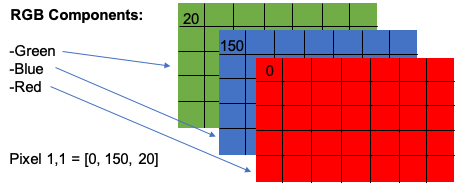
\includegraphics[width=0.9\linewidth]{figures/ch15_pixel.png}
\caption{Representation of the matrix data structure of a RGB image in which each pixel contains information for the intensity of each color component}
\label{fig:pixel}
\end{figure}

The good news when working with digital images is that the concept of \texttt{pixel} (picture element) will help you to understand the basic mathematical representation behind computational analysis of images. A rectangular grid of pixels is represented by a dot matrix which in turn generates a \texttt{bitmap image} or \texttt{raster graphic}. The dot matrix data structure is a basic but powerful representation of the images since we can conduct multiple simple and advanced operations with the matrices. Specifically, each dot in the matrix is a number that contains information about the intensity of each pixel (that commonly ranges from 0 to 255) also known as bit or color depth (figure~\ref{fig:pixel}). This means that the numerical representation of a pixel can have 256 different values being 0 the darkest tone of a given color and 255 the lightest. Keep in mind that if you divide the pixel values by 255 you will have a 0-1 scale to represent the intensity.

In a blank-and-white picture we will only have one color (grayscale), with the darker points representing the black and the lighter ones the white. The mathematical representation will be a single matrix or a two-dimensional array in which the number of rows and columns will correspond to the dimensions of the image. For instance in a 224 x 224 black-and-white picture we will have 50,176 integers (0-255 scales) representing each pixel intensity. 

In \refex{imagel} we convert our original JPG picture to grayscale and then create an object with the mathematical representation (a 453 x 805 matrix).

\pyrex[output=both,caption=Converting images to grayscale and creating a two-dimensional array]{chapter15/imagel}

By contrast, color images will have multiple color channels that depend on the color model you chose. One standard color model is the  three-channel RGB (\textit{red}, \textit{green} and \textit{blue}), but you can find other variations in the chosen colors and the number of channels such as: RYB (\textit{red}, \textit{yellow} and \textit{blue}), RGBA (\textit{red}, \textit{green}, \textit{blue} and \textit{alpha}\footnote{Alpha refers to the opacity of each pixel} ) or CMYK (\textit{cyan}, \textit{magneta}, \textit{yellow} and \textit{key}\footnote{Key refers to \textit{black}}).  Importantly, while schemes used for printing such as CMYK are \emph{substractive} (setting all colors to their highest value results in black, setting them to their lowest value results in white), schemes used for computer and television screens (such as RGB) are \emph{additive}: setting all of the colors to their maximal value results in white (pretty much the opposite as what you got with your paintbox in primary school).

We will mostly use RGB in this book since it is the most used representation in the state-of-the-art literature in computer vision given that normally these color channels yield more accurate models. RGB's mathematical representation will be a three-dimensional matrix or a collection of three two-dimensional arrays (one for each color) as we showed in figure~\ref{fig:pixel}. Then a RGB 224 x 224 picture will have 50,176 pixel intensities for each of the three colors, or in other words a total of 150,528 integers!

Now, in \refex{imagergb} we convert our original JPG file to a RGB object and then create a new object with the mathematical representation (a 453 x 805 x 3 matrix).

\pyrex[output=both,caption=Converting images to RGB color model and creating three two-dimensional arrays]{chapter15/imagergb}

Instead of pixels, there are other ways to store digital images. One of them is the \textit{vector graphics}, with formats such as .ai, .eps, .svg or .drw. Differently to bitmap images, they don't have a grid of dots but a set of \textit{paths} (lines, triangles, square, curvy shapes, etc.) that have a start and end point, so simple and complex images are created with paths. The great advantage of this format is that images do not get "pixeled" when you enlarge them because the paths can easily be transformed 	while remaining smooth. However, to obtain the standard mathematical representation of images you can convert the vector graphics to raster graphics (the way back is a bit more difficult and often only possible by approximation)

Sometimes you need to convert your image to a specific size. For example, in the case of image classification this is a very important step since all the input images of the model must have the same size. For this reason, one of the most common tasks in the preprocessing stage is to change the dimensions of the image in order to adjust width and height to a different size. In \refex{resize} we use tje \fn{resize} method provided by \pkg{pil} and the \fn{image\_scale} function in \pkg{imagemagik} to reduce the first of our original pictures in RGB (\texttt{my\_image1\_RGB}) to 25\% . Notice that we first obtain the original dimensions of the photograph (i.e. \texttt{my\_image1\_RGB.width} or \verb|image_info(my\_image1\_RGB)['width'][[1]]|) and then multiply by 0.25 in order to obtain the new size which is the argument required by the functions.

\pyrex[output=both,format=png,caption=Resize to 25\% and visualize a picture]{chapter15/resize}

Now, using the same functions of the latter example, we specify in \refex{resize2} how to resize the same picture to 224 x 244, which is one of the standard dimensions in computer vision. 

\pyrex[output=both,format=png,caption=Resize to 224 x 224 and visualize a picture]{chapter15/resize2}

You may have noticed that the new image has now the correct width and height but that it looks deformed. The reason is that the original picture was not squared and our order was to forcedly fit it into a 224 x 224 square, loosing its original aspect. There are different alternative to solve this issue, but probably the most extended is to \textit{crop} the original image to create a squared picture. As you can see in \refex{crop} we can create a function that first determines the orientation of the picture (vertical versus horizontal) and then cut the margins (upper and down if it is vertical; and left and right if it is vertical) to create a square. After applying this ad hoc function \fn{crop} to the original image we can resize again to obtain a non-distorted 224 x 224 image.

Of course you are loosing now part of the picture information, so you may think of other alternatives such as filling a couple of sides with blank pixels (or \texttt{padding}) in order to create the square by adding information instead of removing.

\pyrex[output=both,format=png,caption=Function to crop the image to create a square and the resize the picture]{chapter15/crop}

You can also adjust the orientation of the image, flip it, or change its background, among other commands. These techniques might be useful for creating extra images in order to enlarge the training set in image classification (see Section~\ref{sec:cnn}). This is called \textit{data augmentation} and consists for duplicating the initial examples from where the model learn and give them some twist so the algorithm can be more robust and generalize better. In \refex{rotate} we used the \fn{rotate} method in \pkg{pil} and \fn{image\_rotate} function in \pkg{imagemagik} to rotate 45 degrees the above resized image \texttt{my\_image1\_RGB\_224} to see how easy we can get an alternative picture with similar information to include in an augmented training set.

\pyrex[output=both,format=png,caption=Rotating 45 degrees a picture]{chapter15/rotate}

Finally, the numerical representation of visual contents can help us to \textit{compare} pictures in order find similar or even duplicate images. Let's take the case of RGB images which in \refex{imagergb} we showed how to transform into a three two-dimensional array. If we now convert the 3D matrix of the image into a flatten vector we can use use new simpler numerical representation to estimate similarities. Specifically, as we do in \refex{flatten}, we can take the vectors of two \textit{flatten images} of resized 15 x 15 images to ease computation (\texttt{img\_vect1} and \texttt{img\_vect2}) and use the \textit{cosine similarity} to estimate how akin those images are. We stacked the two vectors in a matrix and then used the \fn{cosine\_similarity} function of the \fn{metrics} module of the  \pkg{sklearn} package in Python and the \fn{cosine} function of the \pkg{lsa} package in R.

\pyrex[output=both,caption=Comparing two flatten vectors to detect similarities between images]{chapter15/flatten}
 
As you can notice in the resulting matrix when the images are compared with themselves (that would be the case of an exact duplicate) they obtain a value of 1. Similar images would obtain values under 1 but still close to it, while dissimilar images would obtain low values.
